\documentclass[12pt]{article}
\usepackage[T2A,T1]{fontenc}
\usepackage[utf8]{inputenc}
\usepackage[greek,russian,english]{babel}

\usepackage[landscape,a4paper]{geometry}
\geometry{verbose,tmargin=0cm,bmargin=0cm,lmargin=3cm,rmargin=3cm}

\usepackage{fancybox}
\usepackage{calc}
\usepackage{multicol}
\usepackage{graphicx}
\usepackage{url}
\usepackage{eso-pic}
\usepackage{textcomp}
\usepackage{paratype}
\usepackage{tgpagella}
\usepackage{xcolor}
\usepackage{mathpazo}  % (Optional) For Palatino style math fonts

% If you want a different main sans font:
\renewcommand{\familydefault}{\sfdefault}

% Define custom colors
\definecolor{Orange500}{HTML}{F95C22}
\definecolor{Slate600}{HTML}{20262C}
\definecolor{DarkBlue500}{HTML}{1C4DA1}
\definecolor{GrayLine}{HTML}{858B91}

% Background image command
\newcommand\BackgroundPic{%
  \put(0,0){%
    \parbox[b][\paperheight]{\paperwidth}{%
      \vfill
      \centering
      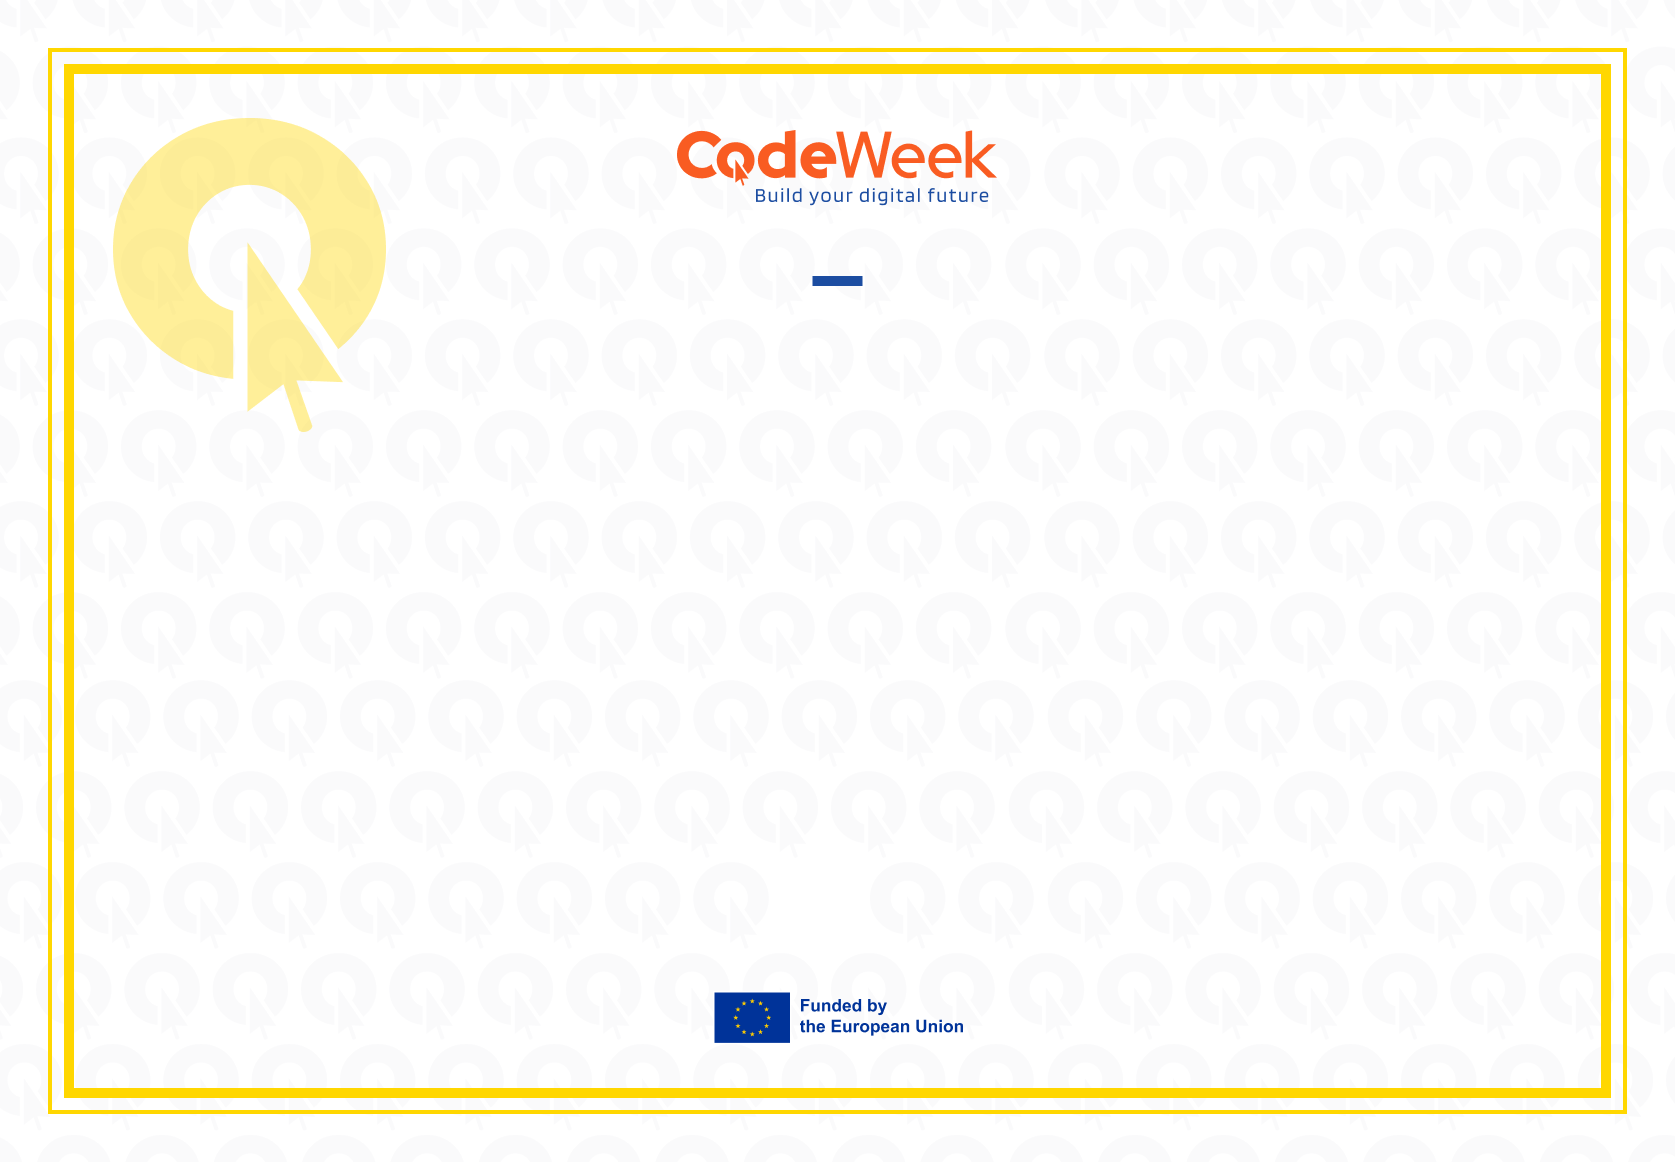
\includegraphics[width=\paperwidth,height=\paperheight,keepaspectratio]{images/super-organiser-2025.png}%
      \vfill
}}}

\begin{document}
\AddToShipoutPicture{\BackgroundPic}

% Some top spacing
~
\vspace{3.5cm}
~
\begin{center}
    \vspace{1.5cm}
    \textcolor{Orange500}{\fontsize{36}{42}\selectfont EU CodeWeek 2024} \\
    \vspace{0.5cm}
    \textcolor{Slate600}{\fontsize{13}{13}\selectfont The European Commission presents this} \\
    \vspace{1cm}
    \textcolor{DarkBlue500}{\fontsize{32}{32}\selectfont Certificate of Super Organiser} \\
    \vspace{0.5cm}
    \textcolor{Slate600}{\fontsize{13}{13}\selectfont To} \\
    \vspace{0.5cm}
    \textcolor{Orange500}{\fontsize{28}{32}\selectfont <CERTIFICATE_HOLDER_NAME>} \\
    \vspace{0.5cm}
    \textcolor{Slate600}{\fontsize{13}{13}\selectfont For Organising} \\
    \vspace{0.5cm}
    \textcolor{DarkBlue500}{\fontsize{20}{20}\selectfont
      \textbf{<NUMBER_OF_ACTIVITIES> coding activities in 2024}
    } \\
    \vspace{1cm}
    \textcolor{Slate600}{\fontsize{13}{13}\selectfont Brussels, <CERTIFICATE_DATE>} \\


\end{center}

\end{document}